\documentclass{article}
\usepackage{graphicx} % Required for inserting images
\usepackage{wrapfig}
\usepackage{subcaption}
\graphicspath{{./images/}}


\usepackage[backend=biber, style=apa, sorting=nyt]{biblatex}
\addbibresource[]{ref.bib}

\title{A study of Swords}
% \author{Thomas Lower}
\date{January 2024}

\begin{document}

\maketitle

\pagebreak

\tableofcontents

\pagebreak

\section{Introduction} \label{intro}
Action and Adventure is one of the largest Genre's within the Cinematic world in terms of Box Office return \parencite{3}. Furthermore, Adventure can be found in the top 3 of all major gaming platforms \parencite{4}. As such, it makes sense to analyse the core of these genres, weaponry. In this article, I intend to focus upon melee weaponry as I find that these offer a healthy balance between animation potential, efficiency to craft and creative possibility. I also intend to specify the weapon as a sword. Due to the well established symbolism associated with the various types of within the current media.

The idea of blades being able to invoke a specific view or feeling is well established within the media world, to the point where the mere concept of a sword and its apparent popularity within media is itself constructed by the media. Within historical times (I will largely be referring to the Medieval era), swords were pretty much exclusively wielded by kings and rulers because of the fact that they were exclusively tools for fighting and served no secondary purpose. Thus, they were extremely rare and more commonly symbolic rather than a common use tool which everyone would know how to use.

Within this, it is my intention to establish a set of symbolisms that a given weapon can portray, and then use photography to successfully capture these symbolic features. Thus, allowing me to reproduce such work in Computer Graphics that would enable more powerful storytelling by allowing specific weapons to be used to provide a given effect within an artistic piece.
\pagebreak


\section{Swords in the media} \label{media}
As mentioned in section \ref{intro}, Films and Video Games that feature melee weaponry are often some of the most popular. Here I will go over a few and their use of these weapons:



\subsection{For Honor}
(\fullcite{forhonor}).
For Honor is a multiplayer fighting game known for its mechanics around stances, allowing any character to hold their weapon in one of three possible stances. An important thing to note for this game is the idea that the weapons are specific to a character - a character who supposedly has specific training, holds specific armour and has specific abilities. This, therefore, implies that these weapons are a part of the characters identity and representation the same as any other aspect. This then presents the idea that weaponry is capable of expressing a specific idea or symbolism, an idea that is found throughout other media.

\subsection{The Elder Scrolls V: Skyrim}
\begin{wrapfigure}{r}{0.25\textwidth}
    \centering
    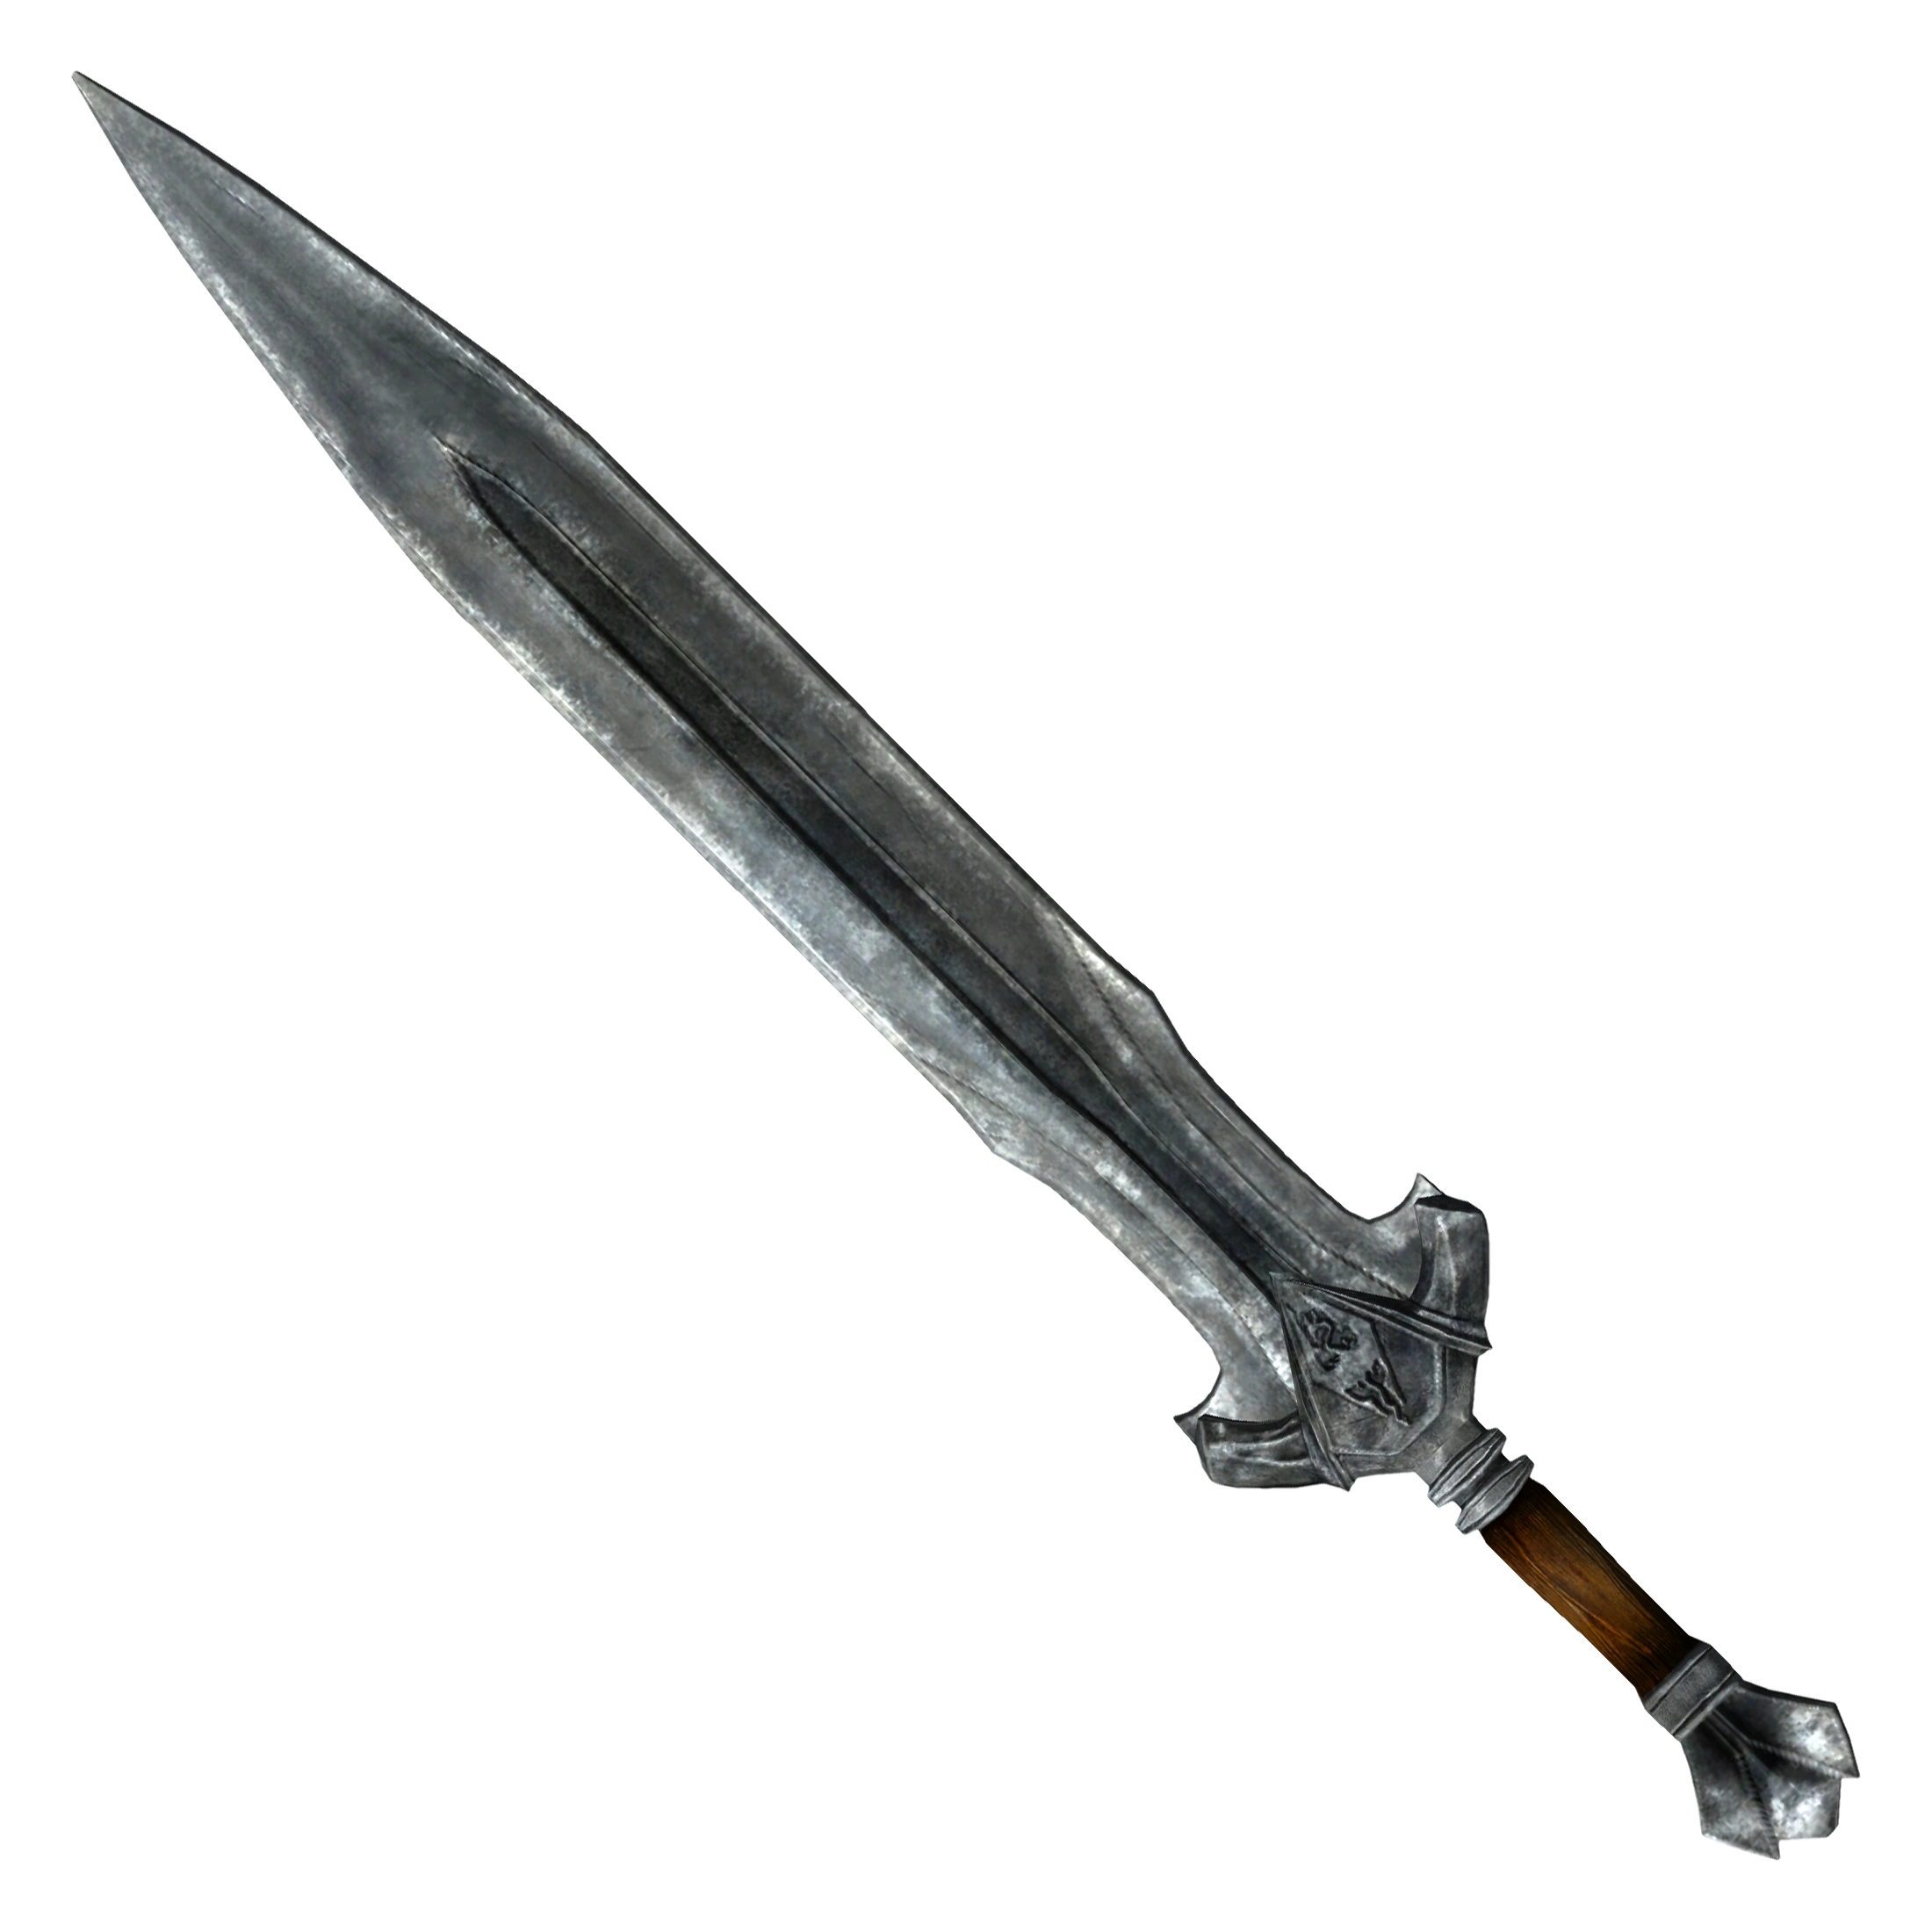
\includegraphics[width=0.25\textwidth]{ImperialSword.png}
    \caption{\parencite{imperialSword} An Imperial Sword from the game "Skyrim".
    }
    \label{fig:ImperialSword}
\end{wrapfigure}
(\fullcite{skyrim}).
Skyrim is a Role Playing Game set in a fantasy setting of its namesake - within the world of Tamreil. This game features multiple different types of sword including the shortsword, longsword and greatsword. However, I feel the most important to note is the first sword encountered by the player in the game - the Imperial shortsword. At the beginning of the game, the player is given a choice to join either the imperial legion or the stormcloak rebellion. The given weapon of the stormcloaks is an axe - typically associated with Viking culture and a brutish mentality which then helps to contrast against the weapon given by joining the imperials, which then helps to give an impression of legality and structure. Such being the common representation of the shortsword.

\pagebreak

\subsection{The Lord of the Rings}

(\fullcite{lotr}).
The Lord of the Rings is both a book and film series set in a medieval fantasy world. Being the generic conventions of the fantasy genre, these feature many different types of swords and blades. The most notable being the dagger held by Bilbo - one of the only magical weapons in the series (to be expected of a dagger as stated in section \ref{daggerSymbol}) as well as the longsword held by Aragorn (which brings its many associations to his own character identity set out in section \ref{longswordSymbol}).

\begin{figure}[h]
    \centering
    \caption{\parencite{Sting} The blade "Sting" from the film "The Hobbit" glowing in the presence of orcs.}
    \label{fig:Sting}
    \includegraphics[width=0.5\textwidth]{Sting.png}
\end{figure}

\pagebreak

\section{Parts and Purpose}
All swords can be broken down into 3 basic components:
\begin{list}{-}{}
    \item A sharp blade which will be used to strike against targets / parry incoming attacks. (see figure \ref{fig:SwordBlade}).
    \item An optional cross guard which blocks an incoming strike from hitting the hand of the wielder. Sometimes also referred to as a handguard or crossbar. (see figure \ref{fig:SwordCross}).
    \item A handle with a size relative to the size of the blade - in units of the size of the hand of a human. (see figure \ref{fig:SwordHandle}).
\end{list}

\begin{figure}[h]
    \centering
    \caption{Pictures of 3 different swords to illustrate their three basic parts}
    \label{fig:PartsOfSwords}
    \begin{subfigure}{0.3\textwidth}
        \includegraphics[width=1\textwidth]{1HandLongswordBlade.jpg}
        \caption{The blade of a one-handed longsword.}
        \label{fig:SwordBlade}
    \end{subfigure}
    \begin{subfigure}{0.3\textwidth}
        \includegraphics[width=1\textwidth]{Saber3Handle.jpg}
        \caption{The golden crossbar of a saber.}
        \label{fig:SwordCross}
    \end{subfigure}
    \begin{subfigure}{0.3\textwidth}
        \includegraphics[width=1\textwidth]{OrnateShortswordHandle.jpg}
        \caption{The handle of an ornate shortsword}
        \label{fig:SwordHandle}
    \end{subfigure}
\end{figure}

The sword of the blade is probably the most crucial - as this is the offensive object of the weapon. The sword blade has multiple different versions with subtle differences.

The sword blade can feature one sharpened edge or two. While the sided blade offers an obvious offensive advantage, this must be balanced with the idea that the blade will therefore require double the maintenance to ensure the blade is properly sharpened, as well as also requiring the blade to be wider. When an object cuts, it uses the sharpened section of the blade to initially separate the object. The width of the blade is then used to push the two new parts further apart and ensure a full cut. This then maximizes blood loss and therefore damage to the target. The effect of bloodloss can then be exemplified by placing a small slit in the centre of the blade for blood to run down (see figure \ref{fig:swordSlit}). 

\begin{figure}[h]
    \centering
    \caption{}
    \begin{subfigure}{0.49\textwidth}
        \includegraphics[width=\textwidth]{SaberDamagedBlade1.jpg}
        \caption{A closeup of the blade showing a crease where the rising parts of the blade meet.}
        \label{fig:SwordCrease}
    \end{subfigure}
    \begin{subfigure}{0.49\textwidth}
        \includegraphics[width=\textwidth]{SpearSide.jpg}
        \caption{The side of a spear to show the slope effect.}
        \label{fig:SpearSide}
    \end{subfigure}
    \begin{subfigure}{\textwidth}
        \centering
        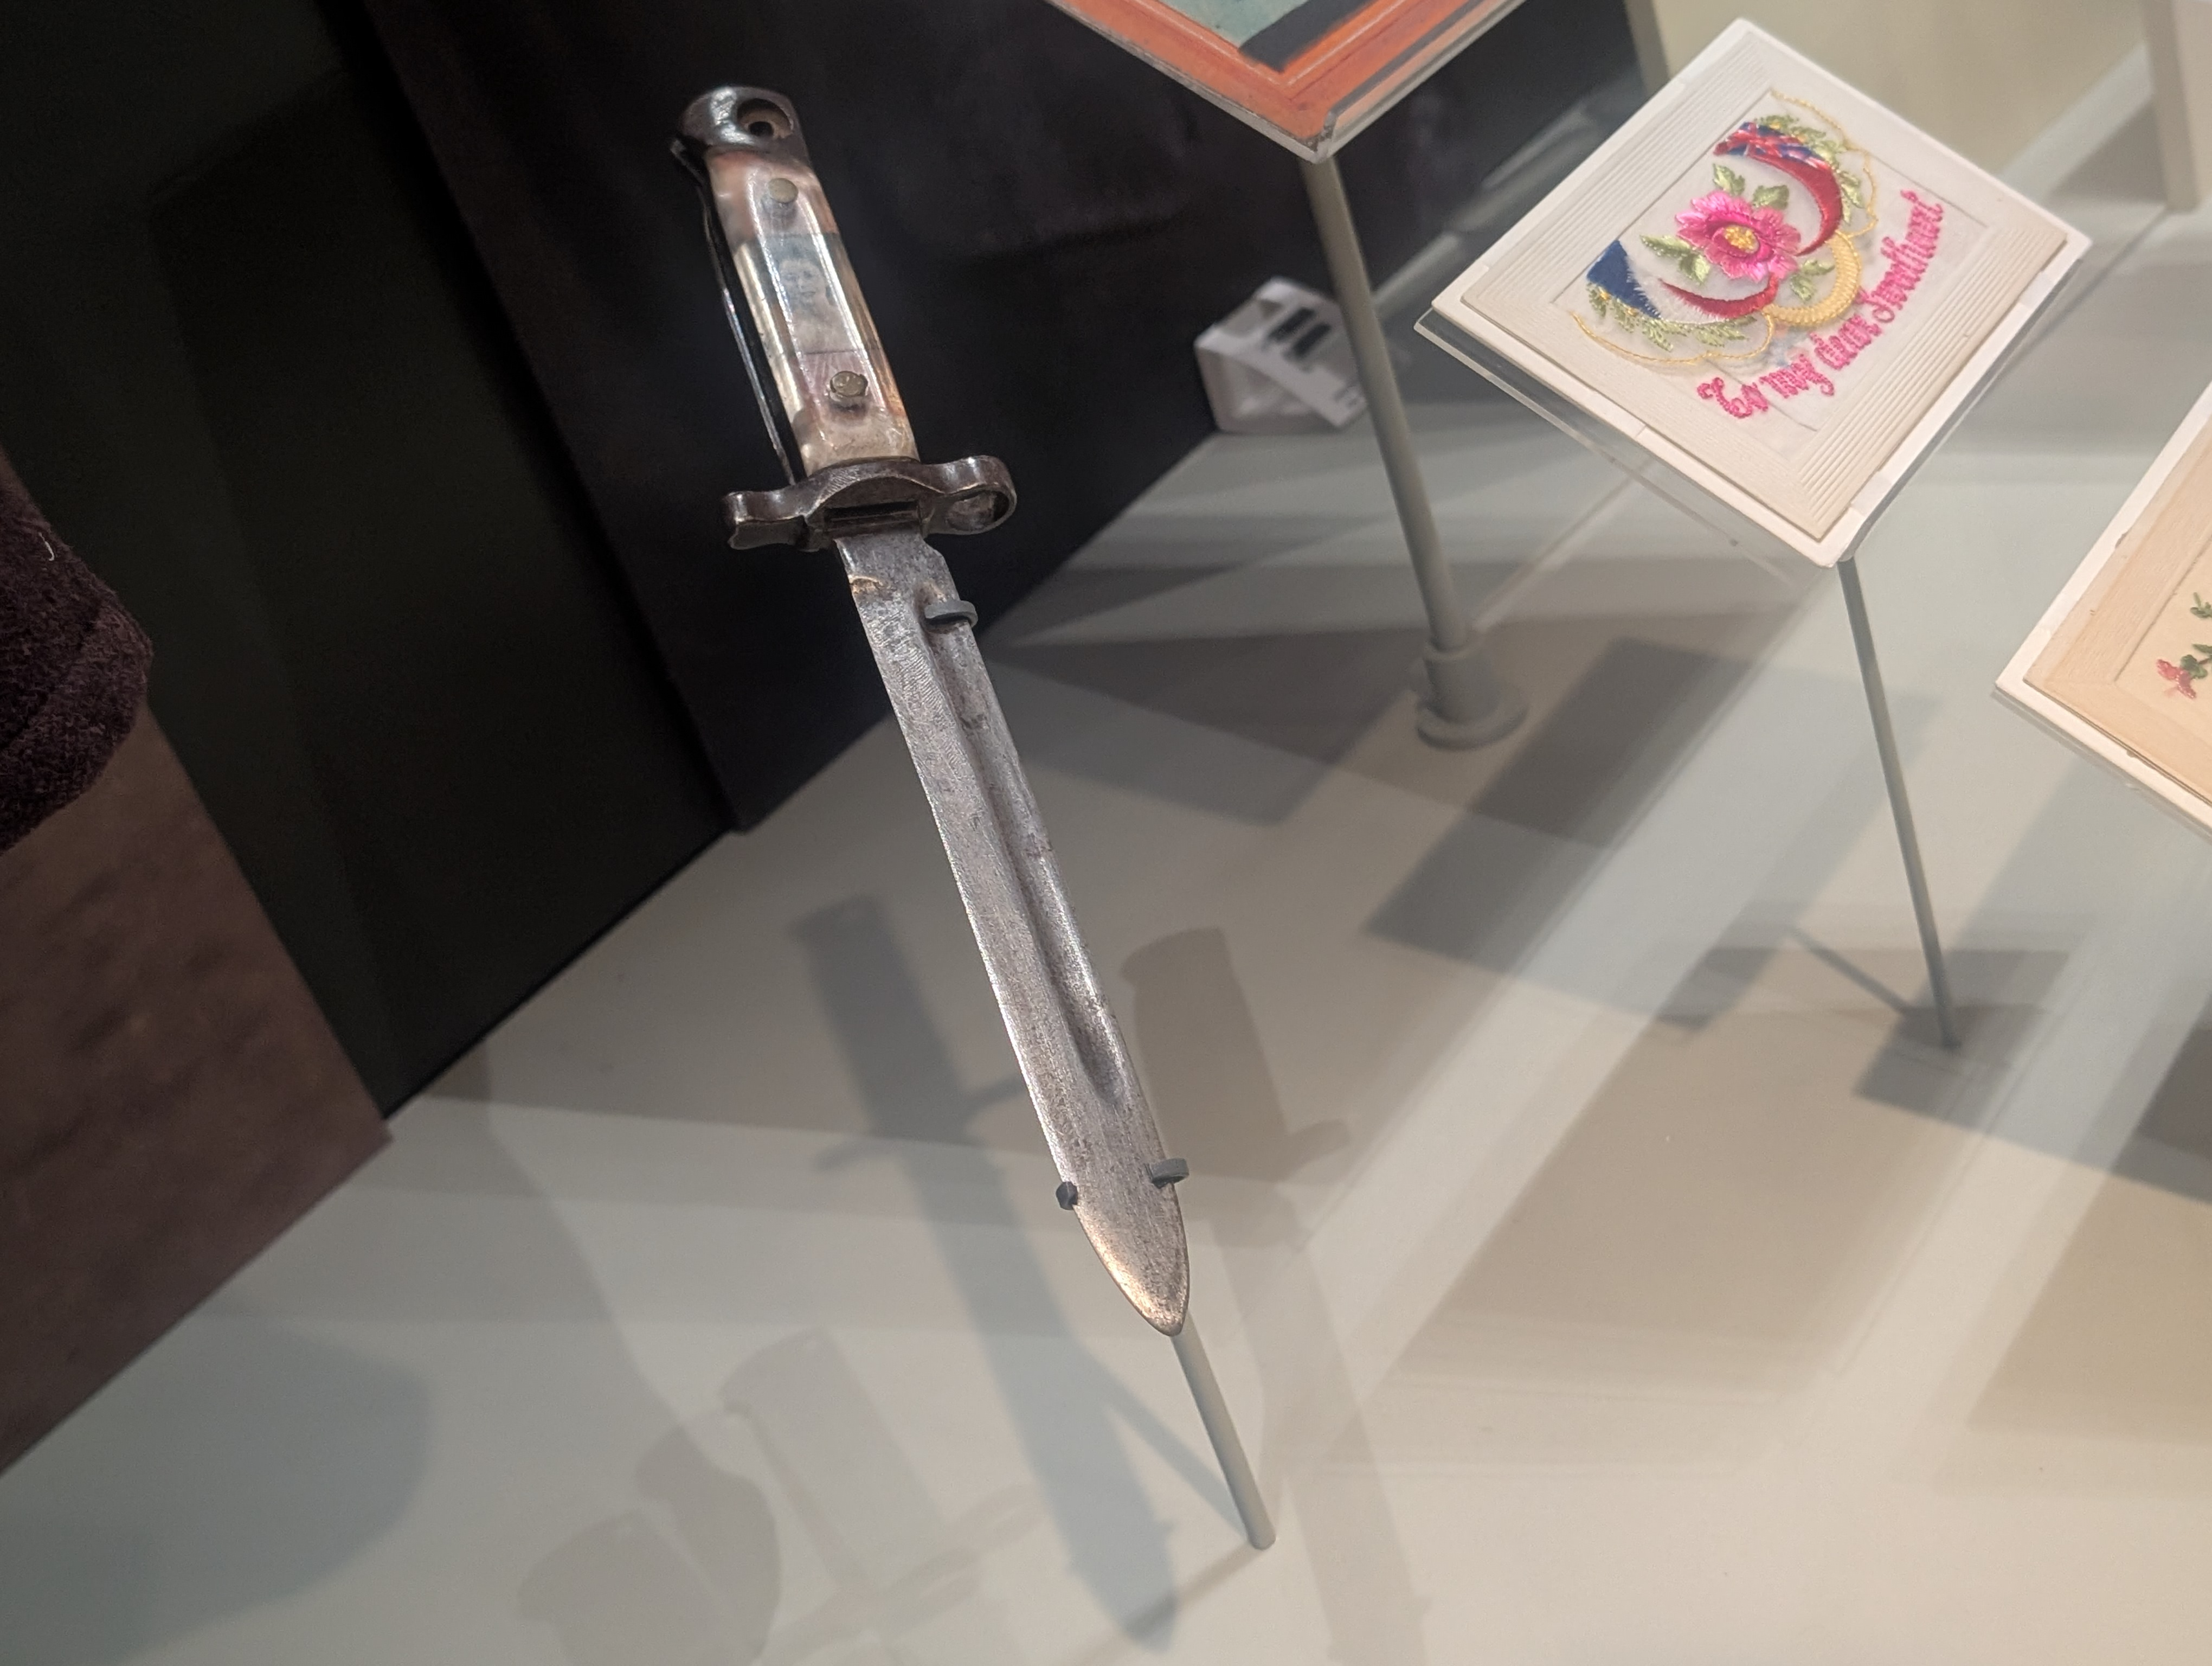
\includegraphics[width=0.5\textwidth]{Dagger2.jpg}
        \caption{A dagger with a slit through which blood can run after stabbing a person to enable a person to more effectively bleed out without having to remove the knife.}
        \label{fig:swordSlit}
    \end{subfigure}
\end{figure}

However, this requires the width of the blade to increase at a certain rate as too high an increase will negatively affect the speed of the blade and its ability to cut effectively (try to imagine the different between cutting with a sharp edge, and cutting with the face of a cube (see this effect in figure \ref{fig:SpearSide})). It is because of this that the blade therefore becomes much wider if having multiple sharp edges which had put a strain on materials. It would have also been a heavier weapon if having multiple blades which, in turn, would therefore become more difficult to wield. This issue can be seen in figure \ref{fig:WideDagger}

\begin{figure}[h]
    \centering
    \includegraphics[width=0.25\textwidth]{LargeBladeDagger.jpg}
    \caption{A Dagger with a wide blade due to its double handedness.}
    \label{fig:WideDagger}
\end{figure}

Another consideration of the number of sharpened edges is the famous "crossed blades" moment in a filmed fight scene. In this 2 characters wielding longswords will become very close and hold their swords against each other - each pressing the blade against each other in an attempt to simply overpower their opponent. During this situation, a combatant would have a clear advantage if they are able to apply pressure to the back of the blade as Archimedes' research on levering would imply that this is a much more effective place to give force to overpower their opponent \parencite{bunn2017archimedes}. This, however, would only be possible on a single edged sword as otherwise the attacker would almost definitely slice their own hand open if they were to press on the other bladed side of a 2 sided blade.

The point of the blade is also of valid importance as some blades will focus towards a singular spike at the edge, while others will fail to do so. The spike at the end opens the blade up to an additional straight - piercing - strike. This strike is much faster and - due to the lack of angular attack - is much more difficult to parry. However, comes at the cost that the bladed edge close to this point becomes somewhat less effective. Above, I mentioned the width of the blade providing an effective method of properly separating the parts of the target which were cut. If the blade focusses into a point though, this width will have to shrink down towards the end of the blade to allow it to form a point, which renders the bladed edge less effective as it loses this separating ability.

\pagebreak

\pagebreak

\section{Sword Symbolism} \label{swordSymbol}
As discussed prior, the term sword is in fact a category to describe many different types of weapons \parencite{furat1998brief}, all of which follow the same general shape pattern of: handle → hand guard → single, continuous blade.
All swords would feature a common representation: that of honour. Within history, most combat would be achieved through armies of levies, who were donated troops from the barons of a kingdom. These troops would not be outfitted by the monarch, but rather, they would outfit themselves with whatever weaponry they could find. Be it scythes, hoes, hatchets or pikes. It would be extremely rare for them to equip a sword as this weapon has no other purpose other than fighting. Thus, it would make no sense for a peasant levy to own a sword. The only people who would battle with swords would be the monarchs and knights of the army; they would be able to afford a sword as well as afford the time to train with it. This is what causes the sword to be commonly associated with honour, as the monarch was \textit{theoretically} the most honourable soldier in the army. Furthermore, this also allows them to serve as a symbol of hope. While the monarch was alive, it could be assumed that you were still winning - or at the very least not losing - the battle. Therefore, if you could see a sword, then you could see your monarch

\subsection{Short sword} \label{shortSwordSymbol}
One of the most basic types of sword, would be more accurately described as a short sword \parencite{mcnab2010swords}. This weapon features a short blade length of no more than 30 cm and often lacks a proper handguard. Thus giving it a sense of aggression as it lacks this key protective implement, requiring the wielder to rely on pure offence in order to overpower their enemies as a posed to being able to fall back to a defensive position when needed. It also requires extreme close range to the target in order to be used effectively, therefore requiring the person holding this weapon to be within direct shot of blood and other gut-like objects when released from the body with this weapon. Which creates an association with it being bloody and brutal as the attacker must be willing to become covered in their enemies blood. Furthermore, it is obvious when somebody wielding this weapon approaches, thus it can be considered bloody and aggressive.

\begin{figure}
    \centering
    \begin{subfigure}{0.33\textwidth}
        \includegraphics[width=\textwidth]{SwordToKillChild2.jpg}
        \caption{A shortsword used when a king threatened to split an infant in half when 2 mothers claimed maternity over the child.}
        \label{fig:killChild}
    \end{subfigure}
    \begin{subfigure}{0.33\textwidth}
        \includegraphics[width=\textwidth]{DavidShortsword.jpg}
        \caption{The shortsword held by David while standing on the decapitated head of Goliath}
        \label{fig:goliathDead}
    \end{subfigure}
    \caption{A collection of shortswords being used in brutish circumstances}
    \label{fig:shortswords}
\end{figure}

\subsection{Dagger} \label{daggerSymbol}
This contrasts greatly to the dagger which would be considered sly and agile. The symbolism related to such a weapon is often that of deceit and mistrust. This is due to its small size and the fact that this allows it to play a crucial part in assassinations. This is true of the real world, such as the death of Julius Caesar \parencite{caesar} in which a character can be seen holding a dagger. As well as in fictional pieces such as Macbeth in which the character Macbeth famously asks: \begin{quote}
    "Is this a dagger I see before me?"
\end{quote}
before stabbing King Duncan \parencite{macbeth}. Therefore, daggers are often associated with evil as they bring about deceitful death against powerful people.

\begin{figure}[h]
    \centering
    \includegraphics[width=1\textwidth]{PersiusWithDagger.jpg}
    \caption{A dagger held by Persius after he slayed Medusa.}
    \label{fig:PersiusDagger}
\end{figure}

Daggers also have a second association, that of the occult. Due to the ease of secrecy as well as the precision - both because of the size of the blade, this weapon is often associated with cult-like rituals that require a donation of blood or other sacrifice. The precision of a dagger allows a participant of such a ritual to control the amount of blood used, such that their life is not at risk from blood loss if it is not supposed to be. This association with brutish occult methods is further enhanced because of the need for the wielder to become very close to their target. This, essentially, makes it impossible for a person to avoid getting the blood and innards of the target on themselves, thus requiring a strong constitution or even appreciation of these otherwise disgusting fluids. Thus leading an association with the occult as those who would practice such rituals are often associated to a lack of remorse around the inner parts and guts of others.

\subsection{Longsword} \label{longswordSymbol}
However, both of these weapons would be considered to be aggressive, demonstrating the lethality of swords. To search for the representation of honour and protection, one must seek the longsword or broadsword. This weapon features a much longer blade, such that it could be comfortably held with two hands, or wielded with one hand if necessary. As well as being featured with a handguard. The size of this weapon allows it to more effectively parry and block, thus allowing it to present as more well-rounded, being capable of slashing at an enemy as well as blocking an attack. This leads to it being the symbol on many coats of arms such as London \parencite{fox1894book} and New York state \parencite{newyorkflag} as it represents adaptability and strength.

\subsection{Rapier}
Now we can begin to discuss more specialized weapons. To begin, lets start with a personal favourite of mine, the rapier. This sword is also commonly referred to as a fencing sword and is characterized by an extremely thin blade - such that it will flop and bend under movement of the handle. It also often features a rounded guard or set of rings that covers the hand or fingers \parencite{walker2002rapier12}. This sword acts as a symbol for one very specific concept, elegance. The rapier is not a slashing weapon like most swords, but rather, exclusively a piercing weapon \parencite{walker2002rapierNoCut}. Such that it uses straight stabs to cause damage to an individual. These straight stabs are designed to be done extremely quickly in extremely precise spots. To wield this weapon therefore requires both attention and intelligence - to know when and where exactly to stab. These requirements lead to the weapon becoming a dedication. Only somebody who is specifically trained with this weapon will be able to use it properly, anyone else will struggle. With this dedication, a certain grace and elegance follows, in both the biological and mathematical knowledge \parencite{walker2002rapier25} to know where to stab, and the form and positioning that is generated to stab swiftly and effectively. Furthermore, This weapon is exclusively offensive as the flimsy of the blade offers no possible defence. However, its lack of weight offers a different approach. With a lightweight weapon that bends to allow easy aerodynamics, plus forming to allow extremely fast movements for stabs, this weapon lends itself well to the agile. This massively supports the idea of elegance as the agility often results in movements that can be quite shocking and interesting to the eye as a wielder dodges and weaves about heavier and less manoeuvrable types of blade.

The association with elegance also originates from its association with the ruling elite, all of whom would wear this weapon as a part of their civil attire - especially in France and Germany within the Middle Ages \parencite{correa2013history}. The simple fact that all of these people would be commonly carrying this weapon led to a strong association with that of elegance as the elegance of the ruling classes became intrinsically attached to the items they carried. This also leads to the more practical symbolism of the rapier - which is that of regal influence and upper class status.

\subsection{Greatsword} \label{greatswordSymbol}
Another important weapon to consider is the \emph{greatsword or claymore}. This weapon is known exclusively for its massive size. Requiring a minimum of 2 hands to even hope to lift it properly. However, this is not enough in most cases. To lift a claymore would, similar to the rapier, require a large amount of training in order to wield it properly. This weapon perhaps offers the opposite symbolism to the rapier. Where the rapier was a symbol of intelligence and agility, where the wielder only needed to pay attention to their own strikes and dodge the enemies. The claymore relies on sheer brutish strength, and timing strikes and swings with the opponent in order to counteract its complete lack of manoeuvrability (bearing in mind that this weapon is often dragged along the ground as its sheer weight is too much to be carried normally). This ultimately leads to an association with strength, but not the same brutish strength that short swords were known for. No, this is an aged and experienced strength, the strength that comes with training and dedication. A strength mixed with awareness and timing, such that the lack of agility of the blade poses no real issue. This practice also leads to a more practical symbolism of the greatsword in the form of age and wisdom - something comparable to the staff of a wizard - due to the practice required by the wielder to achieve strong timing.

It is also worth noting the aggression associated with this weapon, in some part, simply due to its sheer size. But also due to the practice of wielding this weapon. To wield this weapon properly, any movement with the blade should be considered as an attack

\subsection{Sabre} \label{saberSymbol}
The sabre is an important weapon when considering symbolism as it is almost exclusively used as a symbolic artefact rather than a military tool. The design of the sabre follows the curved fashion of the japanese katana however with two key differnces. The katana stills merges to a single point at the end that is capable of piercing, while the sabre curves round to form a shape not dissimilar to that of a banana. Furthermore, the katana is sharpened while the sabre is usually square at its edges (at least in modern day) to avoid a person accidentally harming themselves on the weapon.

Its symbolism is exclusively that of honor and rank. Specifically the honor that could be associated with that of a high ranking general or other military leader as they would be those who are awarded such an item. This explains why many sabres often feature ornate handguards and handles, as well as writing inscribed upon the blades of the swords.

\begin{figure}[h]
\centering
\caption{A collection of images from sabres at the National Army Museum.}
\label{fig:sabreImages}
\begin{subfigure}{0.3\textwidth}
    \includegraphics[width=\textwidth]{Saber4Blade.jpg}
    \caption{An ornate golden sabre with a long inscription}
    \label{fig:Saber4}
\end{subfigure}
\begin{subfigure}{0.3\textwidth}
    \includegraphics[width=\textwidth]{Saber5.jpg}
    \caption{A military sabre}
    \label{fig:Saber5}
\end{subfigure}
\begin{subfigure}{0.3\textwidth}
    \includegraphics[width=\textwidth]{Saber6.jpg}
    \caption{An silver sabre with an engraving along the blade.}
    \label{fig:Saber6}
\end{subfigure}
\begin{subfigure}{0.3\textwidth}
    \includegraphics[width=\textwidth]{Saber2.jpg}
    \caption{A light cavalry troopers sword featuring a sharkskin handle.}
    \label{fig:Saber2}
\end{subfigure}
\begin{subfigure}{0.3\textwidth}
    \includegraphics[width=\textwidth]{Saber3.jpg}
    \caption{An infantry hanger sword given to all privates until 1768.}
    \label{fig:Saber3}
\end{subfigure}
\end{figure}

\pagebreak

\section{Iterations of Sword Symbolism photography}

\subsection{Iteration 1}

\begin{figure}[h]
    \centering
    \caption{}
    \label{fig:Iteration1Imagespt1}
    \begin{subfigure}{0.3\textwidth}
        \includegraphics[width=1\textwidth]{Iteration1.1.jpg}
        \caption{}
        \label{fig:Iteration1.1}
    \end{subfigure}
    \begin{subfigure}{0.3\textwidth}
        \includegraphics[width=1\textwidth]{Iteration1.2.jpg}
        \caption{}
        \label{fig:Iteration1.2}
    \end{subfigure}
\end{figure}
\begin{figure}[h]
    \centering
    \caption{}
    \label{fig:Iteration1Imagespt2}
    \begin{subfigure}{0.35\textwidth}
        \includegraphics[width=1\textwidth]{Iteration1.3.jpg}
        \caption{}
        \label{fig:Iteration1.3}
    \end{subfigure}
    \begin{subfigure}{0.35\textwidth}
        \includegraphics[width=1\textwidth]{Iteration1.4.jpg}
        \caption{}
        \label{fig:Iteration1.4}
    \end{subfigure}
\end{figure}

\pagebreak

The first iteration of attempting to photograph the iconography of swords has positives and flaws. A positive aspect of this iteration is that the regality of the sabre (section \ref{saberSymbol}) is visible within the images (figures \ref{fig:Iteration1.1} and \ref{fig:Iteration1.2}). The gold colourings of the blade as well as the string suspended from the handguard allow for a certain wealth to be exuded from the weapon. Thus allowing it to appear regal. 

However, it is my goal to be able to capture more than this one aspect, which does not occur as the second set of images (figures \ref{fig:Iteration1.3} and \ref{fig:Iteration1.4}) features practically no identifiable iconography or aspects that create any level of symbolism. These two images only contain slight damage to the blade which is otherwise uncharacteristic. It is not particularly clean or dirty, neither features an ornate handguard or particular shape. The weapon is bland and uncharacteristic which disables it from displaying any key symbolic features. While this could be considered a form of symbolism in and of itself, I don't believe it is helpful to my overrall goal. Since I stated this work with the intention of being able to use weapons as a method of narrative (see section \ref{intro}), a lack of characteristics is not itself intrinsically interesting, which would fail to make it useful it portraying a narrative. This ultimately, therefore, must be considered a failure.

\pagebreak

\subsection{Iteration 2}



\pagebreak

\subsection{Iteration 3}



\pagebreak

\printbibliography

\pagebreak

\listoffigures

\end{document}
